\chapter{Metodologia}
\label{chap:metodologia}

O HoTHP (\textit{Hyperbolic Rotary Position Embedding-based Transformer Hawkes Process}) é uma variante do THP que substitui o kernel trigonométrico do RoTHP por um kernel hiperbólico com decaimento exponencial, inspirado no HoPE \cite{dai_hope_2025}. A principal motivação é a extrapolação de comprimento, onde treinamos em sequências curtas e mantemos o desempenho estável em sequências mais longas. O mecanismo por trás dessa capacidade é um viés exponencial de recência embutido diretamente no kernel de atenção, que faz os scores decaírem monotonicamente com a distância temporal, refletindo a estrutura do próprio processo de Hawkes.

\section{A limitação oscilatória do RoTHP}
\label{sec:limitacao-rothp}

Como vimos na Seção \ref{sec:rothp}, o RoTHP representa a posição de cada evento por uma rotação trigonométrica aplicada aos vetores de query $\mathbf{q}$ e key $\mathbf{k}$. O score de atenção entre os eventos $i$ e $j$ depende apenas de $\Delta t = t_i - t_j$, o que é garantido pelas propriedades algébricas da matrize de rotação trigonométrica, que é ortogonal.

O problema é que o kernel resultante é oscilatório. Seno e cosseno não são funções monotônicas. Sendo assim, o score de atenção pode crescer para eventos mais distantes no tempo, dependendo da fase da oscilação, e diminuir para eventos próximos. Isso contradiz diretamente o kernel do processo de Hawkes, $\varphi(\Delta t) = \alpha e^{-\beta \Delta t}$, que é estritamente decrescente.

Na prática, a consequência mais grave dessa oscilação aparece na extrapolação de comprimento. Quando testado em sequências mais longas do que as de treinamento, o modelo encontra diferenças temporais $\Delta t$ que nunca observou durante o treino. Um kernel com decaimento exponencial teria um comportamento previsível nessa região, com a influência continuando a cair. Já o kernel trigonométrico continua oscilando com a mesma amplitude, e um evento muito distante pode receber um score alto simplesmente porque a fase do cosseno caiu em um pico naquele $\Delta t$. O modelo não aprendeu a lidar com essas fases porque nunca as viu durante o treino e o kernel não tem nada que force o score a decair. É essa ausência de viés de recência que impede o RoTHP de extrapolar de forma estável.

\section{Do kernel trigonométrico ao kernel hiperbólico}
\label{sec:trig-to-hyp}

Para cada par de dimensões $(2j{-}1, 2j)$, o RoTHP aplica o bloco $2 \times 2$ de rotação trigonométrica:
%
\begin{equation}
    \mathbf{R}_j(\Delta t) = \begin{bmatrix} \cos(\theta_j \Delta t) & \sin(\theta_j \Delta t) \\ -\sin(\theta_j \Delta t) & \cos(\theta_j \Delta t) \end{bmatrix}.
\end{equation}
%
O HoPE \cite{dai_hope_2025} propõe trocar essa rotação por uma rotação hiperbólica, cujo bloco correspondente é:
%
\begin{equation}
    \mathbf{B}_j(\Delta t) = \begin{bmatrix} \cosh(\theta_j \Delta t) & \sinh(\theta_j \Delta t) \\ \sinh(\theta_j \Delta t) & \cosh(\theta_j \Delta t) \end{bmatrix}.
    \label{eq:bloco-hiperbolico}
\end{equation}
%
Diferentemente de $\cos$ e $\sin$, as funções $\cosh$ e $\sinh$ são monótonas para $\Delta t > 0$, eliminando as oscilações. Entretanto, não podemos usar $\mathbf{B}_j$ diretamente porque a rotação hiperbólica não é ortogonal e o produto interno $\mathbf{q}^\top \mathbf{B}(\Delta t) \mathbf{k}$ \textit{cresce} com $|\Delta t|$ em vez de decair \cite{dai_hope_2025}. Eventos distantes receberiam scores maiores do que eventos próximos, exatamente o oposto do que queremos.

A Figura~\ref{fig:trig-vs-hyp} ilustra essa diferença. No painel esquerdo, $\cos$ e $\sin$ oscilam entre $-1$ e $1$ indefinidamente, sem qualquer tendência de decaimento. No painel direito, $\cosh$ e $\sinh$ eliminam as oscilações mas crescem exponencialmente em ambas as direções. Note que $\cosh$ é uma função par (simétrica, com valor mínimo $\cosh(0) = 1$) enquanto $\sinh$ é ímpar (antissimétrica, com $\sinh(0) = 0$).

\begin{figure}[h!]
    \centering
    \captionsetup{width=14cm}
    \Caption{\label{fig:trig-vs-hyp} Funções base dos kernels de atenção ($\theta = 1{,}0$). Esquerda: funções trigonométricas do RoTHP, que oscilam entre $-1$ e $1$ sem decair. Direita: funções hiperbólicas do HoPE, que são monótonas mas crescem exponencialmente. O crescimento das funções hiperbólicas precisa ser compensado por um fator de decaimento para que o kernel de atenção funcione corretamente.}
    \UFCfig{}{
        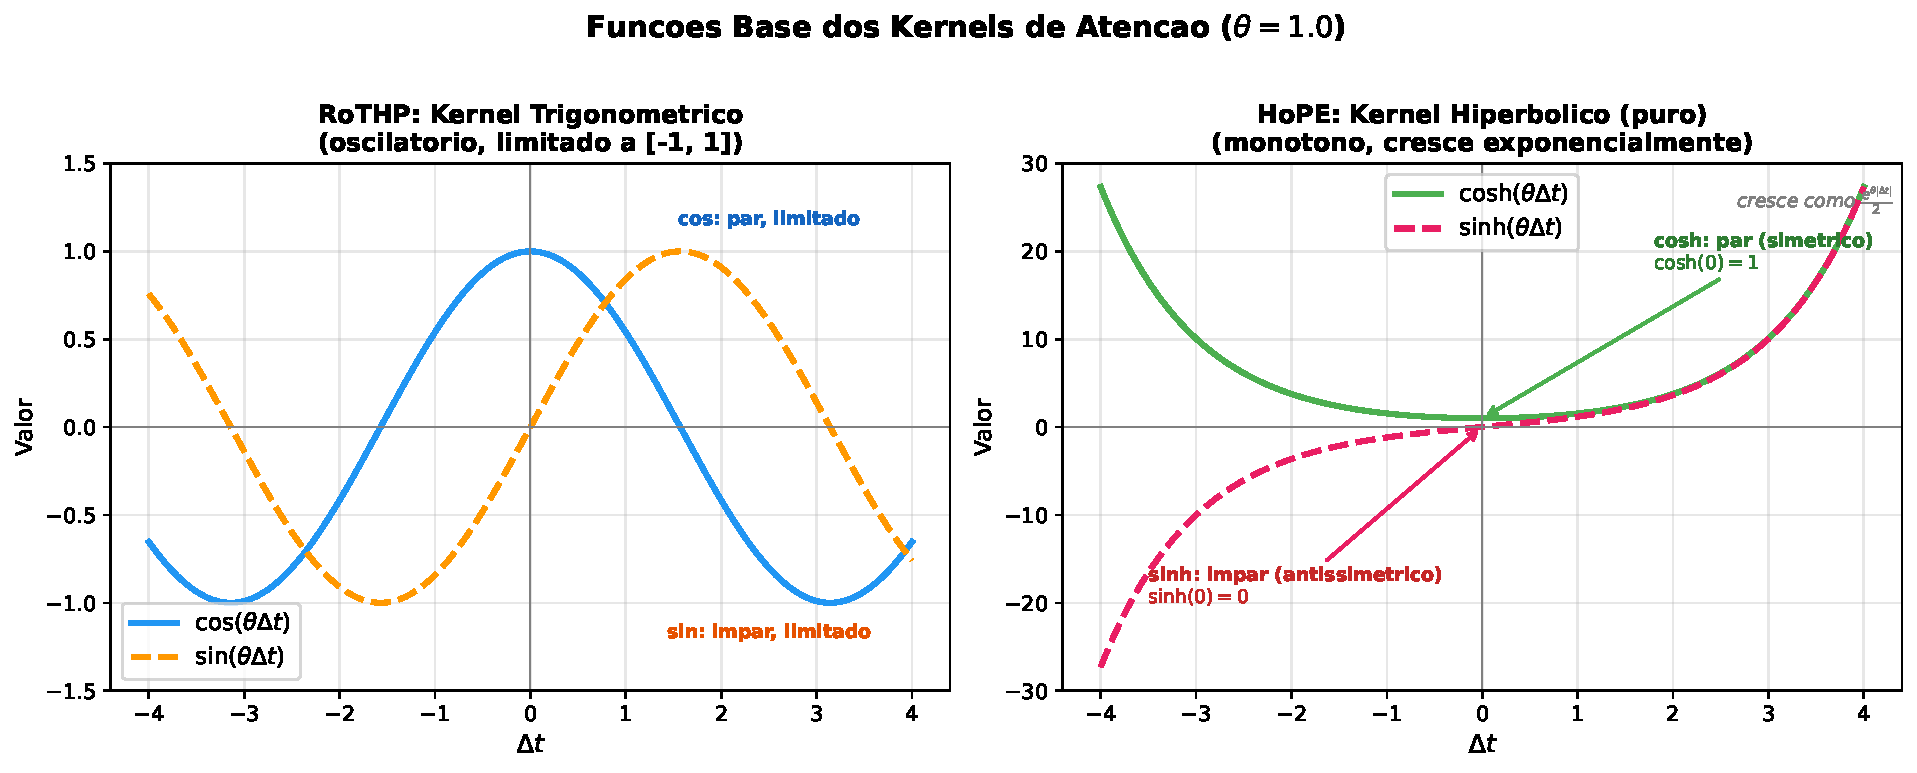
\includegraphics[width=14cm]{figuras/fig_trig_vs_hyp.pdf}
    }{
    }
\end{figure}

\section{Decaimento exponencial e o parâmetro \texorpdfstring{$\theta'$}{theta'}}
\label{sec:decaimento-theta-prime}

Para corrigir o crescimento hiperbólico, o HoPE \cite{dai_hope_2025} introduz um parâmetro aprendível $\theta'$ e aplica fatores de amortecimento nos vetores $\mathbf{q}$ e $\mathbf{k}$. O vetor $\mathbf{q}$ na posição $m$ é multiplicado por $e^{-m\theta'}$ e o vetor $\mathbf{k}$ na posição $n$ é multiplicado por $e^{+n\theta'}$. Ao computar o score entre as posições $m$ e $n$, esses fatores se combinam:
%
\begin{equation}
    g(\mathbf{x}_m, \mathbf{x}_n, n{-}m) = e^{-(m-n)\theta'} \; \mathbf{q}^\top \mathbf{B}(\theta, m{-}n) \; \mathbf{k}.
    \label{eq:hope-score-discreto}
\end{equation}
%
No HoTHP, as posições discretas $m, n$ são substituídas pelos instantes contínuos $t_i, t_j$ e a diferença $m - n$ pela diferença temporal $\Delta t = t_i - t_j$:
%
\begin{equation}
    g(\Delta t) = e^{-\Delta t \cdot \theta'} \; \mathbf{q}^\top \, \mathbf{B}(\theta, \Delta t) \; \mathbf{k}.
    \label{eq:kernel-hothp-completo}
\end{equation}
%
Para que o decaimento domine o crescimento hiperbólico, é necessário que $\theta' > \max_j \theta_j$. Sob essa condição, o score decresce monotonicamente com $|\Delta t|$, o que introduz um viés exponencial de recência no mecanismo de atenção. Esse viés reflete a mesma estrutura do kernel de Hawkes ($\alpha e^{-\beta \Delta t}$) e, por ser estrutural e não aprendido dos dados, vale inclusive para valores de $\Delta t$ que o modelo nunca viu durante o treinamento. É esse viés que dá ao HoTHP a capacidade de extrapolar para sequências mais longas sem degradação.

A Figura~\ref{fig:decay-hiperbolico} ilustra o viés de recência na prática. A imagem da esquerda mostra os componentes separados: $\cosh$ e $\sinh$ crescem exponencialmente enquanto o fator de decaimento $e^{-\theta'\Delta t}$ cai rapidamente para zero. A imagem central mostra o produto das funções hiperbólicas pelo fator de decaimento, garantindo que $\theta' > \theta$, o decaimento domina o crescimento e tanto $e^{-\theta'\Delta t}\cosh(\theta\Delta t)$ quanto $e^{-\theta'\Delta t}\sinh(\theta\Delta t)$ decaem monotonicamente. A imagem da direita mostra a decomposição em exponenciais puras usada na implementação (Seção~\ref{sec:estabilidade-numerica}): como ambos os expoentes $(\theta' - \theta)$ e $(\theta' + \theta)$ são positivos, todas as exponenciais têm argumento negativo e nenhum overflow ocorre.

\begin{figure}[h!]
    \centering
    \captionsetup{width=14cm}
    \Caption{\label{fig:decay-hiperbolico} Efeito do decaimento exponencial sobre as funções hiperbólicas ($\theta = 1{,}0$, $\theta' = 1{,}5$). Esquerda: componentes separados, mostrando que $\cosh$ e $\sinh$ crescem mas o decay cai. Centro: o produto resulta em funções que decaem monotonamente. Direita: decomposição em exponenciais puras, ambas com expoente negativo, garantindo estabilidade numérica.}
    \UFCfig{}{
        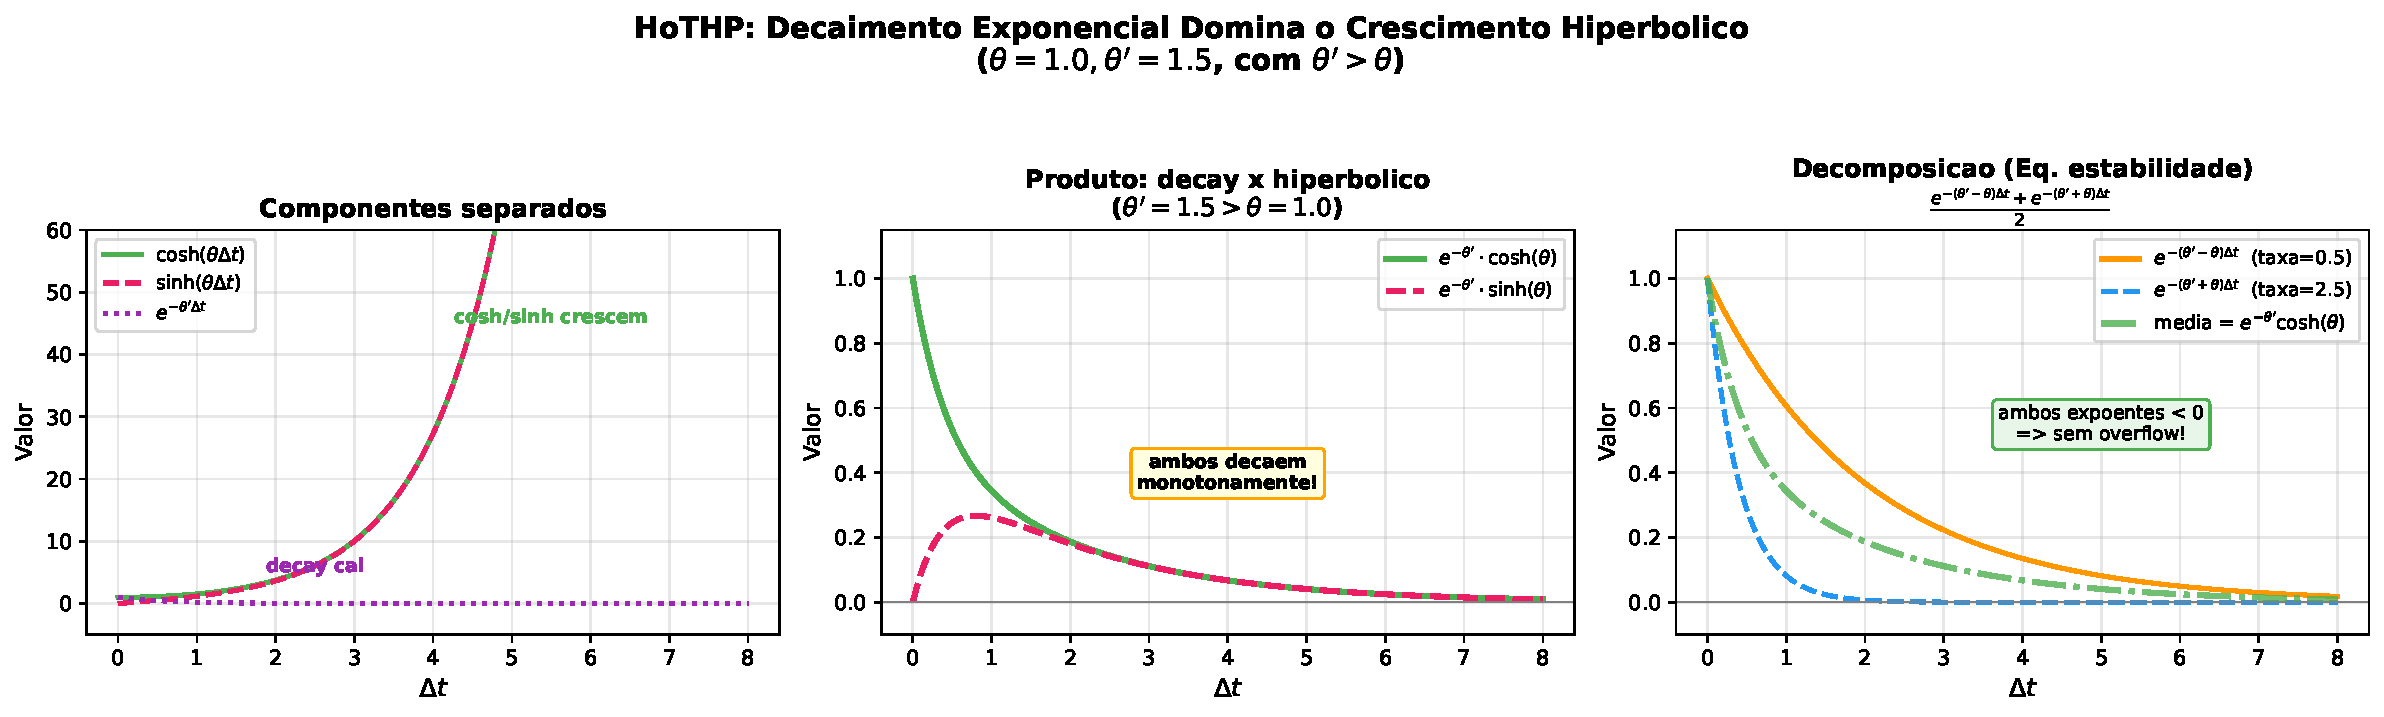
\includegraphics[width=14cm]{figuras/fig_decay_hiperbolico.pdf}
    }{
    }
\end{figure}

\subsection{Parametrização do \texorpdfstring{$\theta'$}{theta'} aprendível}
\label{subsec:parametrizacao-theta-prime}

Como $\theta'$ precisa ser aprendível mas ao mesmo tempo satisfazer $\theta' > \max_j \theta_j$, não podemos simplesmente treinar um parâmetro livre. As frequências $\theta_j$ seguem a fórmula do RoPE \cite{su_roformer_2023}:
%
\begin{equation}
    \theta_j = 10000^{-2(j-1)/d}, \quad j = 1, \ldots, d/2,
    \label{eq:frequencias-theta}
\end{equation}
%
onde $d$ é a dimensão de cada cabeça de atenção. Cada par de dimensões recebe uma frequência diferente, cobrindo múltiplas escalas de $\Delta t$. Note que, pela Equação~\ref{eq:frequencias-theta}, o maior valor de $\theta_j$ ocorre quando $j = 1$, resultando em $\theta_1 = 10000^0 = 1$. Todos os demais $\theta_j$ são frações cada vez menores (por exemplo, $\theta_2 \approx 0{,}013$, $\theta_3 \approx 0{,}00017$, e assim por diante). Portanto, na prática, a restrição $\theta' > \max_j \theta_j$ se resume a garantir que $\theta' > 1$. Ainda assim, optamos por uma formulação geral que funcione independentemente dos valores de $\theta_j$, para que a restrição seja satisfeita por construção. A solução é parametrizar $\theta'$ como:
%
\begin{equation}
    \theta' = \mathrm{softplus}(\theta'_{\mathrm{raw}}) + \max_j(\theta_j) + \epsilon,
    \label{eq:theta-prime-parametrizacao}
\end{equation}
%
onde $\theta'_{\mathrm{raw}}$ é o parâmetro treinável, $\mathrm{softplus}(x) = \ln(1 + e^x)$ garante que o primeiro termo seja positivo e $\epsilon = 10^{-4}$ é uma margem de segurança. Assim, $\theta'$ é sempre maior do que qualquer $\theta_j$ e o decaimento exponencial é garantido estruturalmente, independentemente do que o gradiente faça.

\section{Score de atenção do HoTHP}
\label{sec:score-atencao-hothp}

Expandindo a multiplicação matricial de $\mathbf{B}_j$ (Equação \ref{eq:bloco-hiperbolico}) sobre os vetores de dimensões pares $\mathbf{q}_1, \mathbf{k}_1$ e ímpares $\mathbf{q}_2, \mathbf{k}_2$, obtemos:
%
\begin{equation}
    \mathbf{q}^\top \mathbf{B}_j(\Delta t) \mathbf{k}
    = \underbrace{(\mathbf{q}_1 \cdot \mathbf{k}_1 + \mathbf{q}_2 \cdot \mathbf{k}_2)}_{\text{parte cosh}} \cdot \cosh(\theta_j \Delta t)
    + \underbrace{(\mathbf{q}_1 \cdot \mathbf{k}_2 + \mathbf{q}_2 \cdot \mathbf{k}_1)}_{\text{parte sinh}} \cdot \sinh(\theta_j \Delta t).
    \label{eq:score-par-dimensoes}
\end{equation}
%
O score completo incorpora o fator de decaimento e soma sobre os $d/2$ pares de dimensões:
%
\begin{equation}
    s_{ij} = \frac{1}{\sqrt{d}} \sum_{j=1}^{d/2}
    \left[
        (q_{1}^{(j)} k_{1}^{(j)} + q_{2}^{(j)} k_{2}^{(j)}) \cdot e^{-|\Delta t|\theta'} \cosh(\theta_j \Delta t)
        + (q_{1}^{(j)} k_{2}^{(j)} + q_{2}^{(j)} k_{1}^{(j)}) \cdot e^{-|\Delta t|\theta'} \sinh(\theta_j \Delta t)
    \right],
    \label{eq:score-hothp-completo}
\end{equation}
%
onde $\Delta t = t_i - t_j$ e $1/\sqrt{d}$ é a normalização padrão do \textit{scaled dot-product attention} \cite{vaswani_attention_2017}.

No RoTHP, os vetores $\mathbf{q}$ e $\mathbf{k}$ são pré-rotacionados individualmente por $\mathbf{R}(t_i)$ e $\mathbf{R}(t_j)$ antes do produto interno e a dependência em $\Delta t$ emerge do cancelamento algébrico, demonstrado pelos autores. No HoTHP, o score é formulado diretamente em termos de $\Delta t$, o que torna natural e necessário incluir o fator $e^{-|\Delta t|\theta'}$ dentro do próprio kernel. A consequência prática é que, para qualquer $\Delta t$ (incluindo valores maiores do que os vistos no treino), o score é dominado pelo decaimento exponencial. Esse é o mecanismo que permite a extrapolação: o viés de recência não depende dos dados, ele está na estrutura da atenção.

\section{Estabilidade numérica}
\label{sec:estabilidade-numerica}

As funções $\cosh$ e $\sinh$ crescem como $e^{|\Delta t|\theta_j}$ e para eventos muito espaçados esses valores podem causar \textit{overflow} antes mesmo de serem multiplicados pelo fator de decaimento $e^{-|\Delta t|\theta'}$.

A solução é distribuir o decaimento para dentro das funções hiperbólicas usando as identidades:
%
\begin{align}
    e^{-|\Delta t|\theta'} \cdot \cosh(|\Delta t|\theta_j)
    &= \frac{e^{-|\Delta t|(\theta' - \theta_j)} + e^{-|\Delta t|(\theta' + \theta_j)}}{2},
    \label{eq:decay-cosh}\\[4pt]
    e^{-|\Delta t|\theta'} \cdot \sinh(\Delta t \cdot \theta_j)
    &= \mathrm{sgn}(\Delta t) \cdot \frac{e^{-|\Delta t|(\theta' - \theta_j)} - e^{-|\Delta t|(\theta' + \theta_j)}}{2}.
    \label{eq:decay-sinh}
\end{align}
%
Como $\theta' > \max_j \theta_j$, temos $\theta' - \theta_j > 0$ e $\theta' + \theta_j > 0$, portanto ambos os expoentes são negativos para qualquer $\Delta t$ e o \textit{overflow} não ocorre. O sinal de $\Delta t$ é reintroduzido explicitamente por $\mathrm{sgn}(\Delta t)$, pois $\sinh(-x) = -\sinh(x)$.

\section{Normalização temporal}
\label{sec:normalizacao-temporal}

Datasets diferentes têm escalas temporais muito distintas. Em redes sociais, os intervalos entre eventos podem estar na ordem de milissegundos, enquanto em dados sísmicos ficam na ordem de dias. Se usássemos os instantes brutos no kernel hiperbólico, os valores de $\theta_j \Delta t$ estariam em escalas incompatíveis e o modelo precisaria de hiperparâmetros específicos para cada dataset.

Para evitar isso, aplicamos duas transformações a cada sequência. Primeiro, deslocamos os instantes de modo que a sequência comece em zero e, em seguida, dividimos todos os instantes pela média dos intervalos inter-evento daquela sequência:
%
\begin{equation}
    \tilde{t}_i = \frac{t_i - t_1}{\bar{g}},
    \label{eq:normalizacao-temporal}
\end{equation}
%
onde $\bar{g}$ é a média aritmética dos intervalos entre eventos consecutivos da sequência. Essa operação é feita independentemente para cada sequência. O deslocamento garante que $\tilde{t}_1 = 0$ e a divisão por $\bar{g}$ faz com que o intervalo médio entre eventos passe a ser aproximadamente 1 em todas as sequências, independentemente da escala temporal original do dataset. A ordem e a proporção entre os intervalos são preservadas.

A escolha dessa normalização foi feita após avaliarmos duas alternativas. A primeira foi uma normalização MinMax aplicada aos \emph{intervalos} entre eventos, e não aos instantes absolutos: cada $\Delta t_i = t_i - t_{i-1}$ é mapeado para o intervalo $[0, 1]$ por $\Delta\tilde{t}_i = (\Delta t_i - \Delta t_{\min}) / (\Delta t_{\max} - \Delta t_{\min})$, onde $\Delta t_{\min}$ e $\Delta t_{\max}$ são o menor e o maior intervalo da sequência. Aplicar o MinMax diretamente aos instantes absolutos seria inadequado, pois o último evento é sempre o máximo e, à medida que a sequência cresce, todos os instantes anteriores são empurrados para perto de zero; normalizar os intervalos evita esse problema. Ainda assim, essa alternativa mostrou-se inadequada para o protocolo \textit{train-short, test-long}: nos experimentos sintéticos de extrapolação ela favoreceu sistematicamente o NHP, que não depende de embeddings posicionais explícitos, enquanto os modelos com atenção temporal (THP, RoTHP e HoTHP) foram prejudicados ou apresentaram instabilidade, sobretudo nos fatores de extrapolação elevados.

A razão é que o divisor do MinMax depende do intervalo \emph{máximo} da sequência, e o máximo é um valor extremo que tende a crescer quanto mais eventos a sequência tem, pois sequências mais longas têm maior chance de conter um intervalo atipicamente grande. A normalização por média não sofre desse problema porque o divisor $\bar{g}$ é a média dos intervalos, uma estatística estável que praticamente não muda ao adicionar mais eventos de um mesmo processo: o intervalo médio normalizado permanece $\approx 1$ em qualquer comprimento. Um intervalo atípico também é diluído pela média, ao passo que no MinMax ele alteraria o máximo e comprimiria todos os demais.


A segunda alternativa avaliada foi um fator de escala temporal aprendido como parâmetro do modelo durante o treinamento. Essa abordagem introduziu instabilidade na otimização, com alta variância entre sementes nos fatores de extrapolação elevados. A normalização por média dos intervalos, por ser simples e não depender do comprimento da sequência de teste, foi adotada nos experimentos com dados sintéticos e na ablação do Retweet (Seção~\ref{sec:ablacao-retweet}).

\section{Arquitetura completa}
\label{sec:arquitetura-hothp}

A arquitetura do HoTHP segue o encoder do Transformer \cite{vaswani_attention_2017}. Cada evento $(t_i, k_i)$ é representado por um embedding de tipo aprendível $\mathbf{e}_{k_i} \in \mathbb{R}^d$. Ao contrário do THP \cite{zuo_transformer_2021}, que soma um encoding sinusoidal do tempo absoluto ao embedding, o HoTHP não inclui nenhuma informação temporal no embedding. Os instantes $t_i$ entram no modelo apenas pelo kernel hiperbólico.

O modelo empilha $N$ camadas de encoder hiperbólico, cada uma com um bloco de atenção multi-head hiperbólica seguido de uma rede \textit{feed-forward}. A atenção computa os scores via Equação \ref{eq:score-hothp-completo}, usando as diferenças normalizadas $\Delta\tilde{t}_{ij} = \tilde{t}_i - \tilde{t}_j$. Uma máscara causal garante que cada evento atenda apenas a eventos anteriores.

A rede \textit{feed-forward} em cada camada tem duas projeções lineares com ReLU entre elas:
%
\begin{equation}
    \mathrm{FFN}(\mathbf{x}) = \mathbf{W}_2 \cdot \mathrm{ReLU}(\mathbf{W}_1 \mathbf{x} + \mathbf{b}_1) + \mathbf{b}_2,
\end{equation}
%
com dimensão interna $2d$. Assim como o RoTHP \cite{dai_rotary_2026}, o HoTHP não usa conexões residuais (add \& norm).

A saída do encoder $\mathbf{h}(t_j) \in \mathbb{R}^d$ para o evento $j$ é usada para calcular a intensidade condicional de cada tipo $k$ no instante $t > t_j$:
%
\begin{equation}
    \lambda_k(t \mid \mathcal{H}_t)
    = \mathrm{softplus}\!\left(
        \alpha_k \frac{t - t_j}{t_j + \epsilon}
        + \mathbf{w}_k^\top \mathbf{h}(t_j)
        + b_k
    \right),
    \label{eq:intensidade-hothp}
\end{equation}
%
onde $\alpha_k$, $\mathbf{w}_k$ e $b_k$ são parâmetros aprendíveis e $\mathrm{softplus}$ garante que a intensidade seja positiva. O termo $\alpha_k (t - t_j) / t_j$ captura a variação com o tempo desde o último evento, e $\mathbf{w}_k^\top \mathbf{h}(t_j)$ traz o contexto histórico do encoder. Essa forma segue o THP \cite{zuo_transformer_2021}.

\section{Onde atua o viés exponencial}
\label{sec:onde-atua-vies}

Uma distinção importante precisa ser feita sobre o papel do decaimento exponencial no HoTHP. O fator $e^{-|\Delta t|\theta'}$ não atua diretamente na função de intensidade $\lambda_k(t)$, e sim no mecanismo de atenção que produz o estado oculto $\mathbf{h}(t_j)$. Essas são duas etapas distintas do modelo, com papéis diferentes:

\begin{enumerate}
    \item \textbf{Atenção hiperbólica} (Equação~\ref{eq:score-hothp-completo}): determina os pesos com que cada evento passado contribui para o estado oculto. O decaimento exponencial faz com que eventos recentes recebam pesos maiores e eventos distantes recebam pesos próximos de zero. O resultado é o vetor $\mathbf{h}(t_j)$, que codifica o contexto histórico da sequência.

    \item \textbf{Função de intensidade} (Equação~\ref{eq:intensidade-hothp}): usa o estado oculto $\mathbf{h}(t_j)$ e o tempo decorrido desde o último evento para calcular $\lambda_k(t)$. O parâmetro $\alpha_k$ nessa equação é aprendível e pode assumir valores positivos ou negativos. Se $\alpha_k > 0$, a intensidade cresce com o tempo desde o último evento, caracterizando um processo auto-inibitório. Se $\alpha_k < 0$, a intensidade diminui, como em um processo de Hawkes auto-excitante clássico.
\end{enumerate}

Essa separação tem uma consequência importante que é o fazer com que o viés exponencial do HoTHP não imponha que o processo modelado seja auto-excitante. O kernel hiperbólico impõe apenas que a relevância dos eventos passados para a construção do estado oculto decaia exponencialmente com a distância temporal. A dinâmica da intensidade em si (se ela sobe ou desce após um evento) é determinada pelos parâmetros aprendíveis da camada de intensidade, que são livres para se adaptar aos dados.

Portanto, o HoTHP é adequado para qualquer processo pontual em que o evento mais recente carregue mais informação do que eventos distantes para prever o próximo. Isso inclui tanto processos auto-excitantes (onde eventos geram mais eventos próximos) quanto auto-inibitórios (onde a ocorrência de um evento reduz temporariamente a probabilidade de novos eventos). O viés é prejudicial quando eventos distantes são tão ou mais relevantes que os recentes, como em processos sem memória temporal ou com dependências de longo alcance.

A Figura~\ref{fig:kernel-rothp-vs-hothp} sintetiza visualmente a diferença entre os kernels de atenção do RoTHP e do HoTHP. Na zona de treino (fundo verde), ambos os modelos observam as mesmas distâncias temporais e podem aprender pesos de atenção adequados. Na zona de extrapolação (fundo vermelho), o kernel trigonométrico do RoTHP continua oscilando em fases que o modelo nunca viu durante o treino, atribuindo scores potencialmente altos a eventos muito distantes. O kernel hiperbólico do HoTHP, por outro lado, decai monotonicamente para zero independentemente da distância, graças ao viés estrutural. Para referência, a curva tracejada mostra o kernel de Hawkes clássico ($e^{-\beta \Delta t}$), cuja forma o HoTHP reproduz pela própria arquitetura.

\begin{figure}[h!]
    \centering
    \captionsetup{width=14cm}
    \Caption{\label{fig:kernel-rothp-vs-hothp} Comparação dos kernels de atenção em função da distância temporal $\Delta t$. Na zona de treino, ambos os modelos podem se ajustar aos dados. Na zona de extrapolação, o kernel trigonométrico do RoTHP oscila em fases não aprendidas, enquanto o kernel hiperbólico do HoTHP decai monotonicamente, como o kernel de Hawkes clássico.}
    \UFCfig{}{
        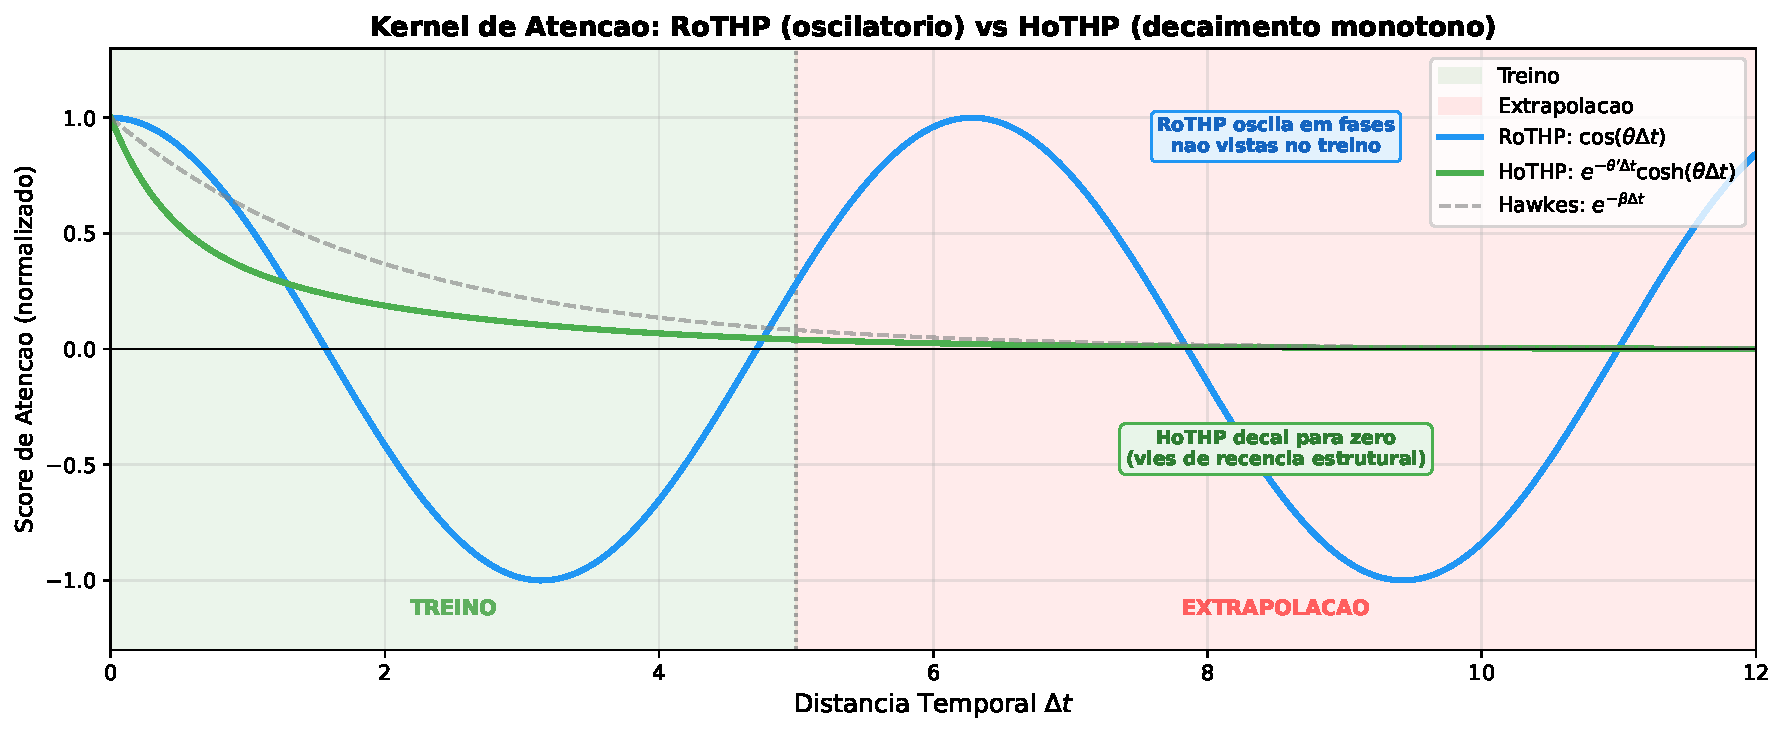
\includegraphics[width=14cm]{figuras/fig_kernel_rothp_vs_hothp.pdf}
    }{
    }
\end{figure}

\section{Configuração experimental}
\label{sec:configuracao-experimental}

Os experimentos utilizam dois tipos de dados: sintéticos e reais. Os dados sintéticos são gerados por processos de Hawkes com kernel exponencial. A escolha de dados sintéticos é deliberada: como conhecemos o processo gerador, podemos verificar se o viés de recência do HoTHP de fato se alinha com o decaimento real dos dados e se essa correspondência é o que sustenta a extrapolação. Os dados reais são os datasets disponibilizados pela biblioteca EasyTPP \cite{xue_easytpp_2024}: Taxi, StackOverflow, Retweet e Amazon. Esses datasets cobrem domínios variados (transporte, fóruns de perguntas, redes sociais e comércio eletrônico) e permitem avaliar o desempenho do HoTHP em cenários onde o processo gerador é desconhecido.

\subsection{Geração de dados sintéticos}
\label{subsec:geracao-dados}

Geramos sequências de processos de Hawkes multivariados com $K = 2$ tipos de evento e kernel exponencial. Definimos dois cenários de geração para cobrir regimes distintos de dependência temporal.

No \textbf{cenário de decaimento lento}, o parâmetro $\beta$ é pequeno, de modo que a influência de eventos passados persiste por mais tempo e eventos distantes ainda afetam a intensidade presente.

No \textbf{cenário de decaimento rápido}, $\beta$ é grande e apenas eventos recentes têm influência relevante.

Para cada cenário, geramos 400 sequências de treinamento, 100 de validação e 200 de teste. Todas as sequências são pré-processadas com a normalização temporal da Equação~\ref{eq:normalizacao-temporal} antes de alimentar os modelos.

\subsection{Protocolo \textit{train short, test long}}
\label{subsec:train-short-test-long}

O protocolo \textit{train short, test long}, proposto por \citeonline{press_train_2021} para modelos de linguagem, treina o modelo em sequências curtas e o testa em sequências mais longas. Adaptamos o protocolo para processos pontuais usando o número de eventos como medida de comprimento.

Fixamos o comprimento de treinamento em $L = 50$ eventos e variamos o fator de extrapolação em $\{1\times, 2\times, 5\times, 10\times\}$, onde o fator indica quantas vezes a sequência de teste é mais longa do que a de treinamento. Com fator $10\times$, por exemplo, treinamos com sequências de 50 eventos e testamos com sequências de 500. Cada fator é avaliado nos dois cenários de decaimento.

\subsection{Modelos comparados e implementação}
\label{subsec:modelos-comparados}

Nos dados sintéticos comparamos quatro modelos: NHP \cite{mei_neural_2017}, THP \cite{zuo_transformer_2021}, RoTHP \cite{dai_rotary_2026} e o HoTHP proposto. O RoTHP é o baseline mais próximo, pois compartilha exatamente a mesma estrutura de encoder e a mesma função de intensidade do HoTHP, diferindo apenas no kernel posicional; o NHP (recorrente) e o THP (encoding temporal absoluto) servem para situar o comportamento na extrapolação em relação a arquiteturas distintas. Nos dados reais comparamos THP, RoTHP e HoTHP no Amazon e no Stackoverflow, e RoTHP e HoTHP no Taxi e no Retweet.

Todos os modelos são implementados no framework EasyTPP \cite{xue_easytpp_2024}, e os baselines compartilham os mesmos hiperparâmetros do HoTHP em cada cenário, de modo a isolar o efeito do kernel posicional. Nos experimentos sintéticos usamos dimensão do modelo $d = 32$, dimensão do \textit{embedding} temporal igual a $32$, $N_{\ell} = 2$ camadas, $H = 2$ cabeças de atenção, \textit{dropout} de $0{,}1$ e otimizador AdamW (\textit{weight decay} $10^{-4}$) com taxa de aprendizado $10^{-3}$, exceto o HoTHP, que usa $5 \times 10^{-4}$ para maior estabilidade numérica das funções hiperbólicas. Nos experimentos com dados reais usamos $d = 64$, \textit{embedding} temporal igual a $16$, $N_{\ell} = 2$ camadas, $H = 2$ cabeças e taxa de aprendizado $10^{-3}$ para todos os modelos.

\subsection{Métricas e avaliação estatística}
\label{subsec:metricas}

A métrica de avaliação é a \gls{NLL}, calculada sobre a sequência completa de teste, incluindo os eventos além do comprimento de treinamento. Se o viés de recência do HoTHP de fato habilita a extrapolação, a NLL deve se manter estável mesmo quando a sequência de teste é muito mais longa do que a de treino. Utilizamos também RMSE para avaliar a predição do próximo evento e Acurácia para avaliar predição do tipo do próximo evento.

Repetimos os experimentos sintéticos com $N = 10$ seeds e os experimentos com dados reais com $N = 3$ seeds, reportando média $\pm$ desvio padrão. Para verificar significância estatística nos experimentos sintéticos, usamos o teste de Wilcoxon de postos sinalizados (\textit{Wilcoxon signed-rank test}), um teste não paramétrico pareado que não assume normalidade e é adequado para amostras pequenas. O pareamento é por semente: a mesma semente gera o mesmo conjunto de treino, validação e teste para todos os modelos. Com $N = 10$, o menor $p$-valor unilateral atingível é $1/2^{10} \approx 0{,}001$, suficiente para o nível $\alpha = 0{,}05$.

\subsection{Ambiente computacional}
\label{subsec:ambiente-computacional}

Todos os experimentos foram executados em uma máquina com GPU NVIDIA A100-SXM4-80GB (80~GB de VRAM), 6 núcleos físicos (12 threads), 167~GB de RAM e CUDA 12.8. O código utiliza PyTorch 2.10.0 e Python 3.12.